\let\lesson\undefined
\newcommand{\lesson}{\phantomlesson{Bài 5.}}
\section{Bài tập trắc nghiệm}
\begin{enumerate}[label=\bfseries Câu \arabic*:, leftmargin=1.7cm]
	\item \mkstar{1}\\
	Tập hợp ba thông số xác định trạng thái của một lượng khí xác định là
	\begin{mcq}(2)
		\item áp suất, thể tích, khối lượng.
		\item áp suất, nhiệt độ, thể tích.
		\item thể tích, trọng lượng, áp suất.
		\item áp suất, nhiệt độ, số mole.
	\end{mcq}
\hideall{
\textbf{Đáp án B.}
}

\item \mkstar{1}\\
Quá trình đẳng nhiệt là
\begin{mcq}
	\item quá trình biến đổi trạng thái của một lượng khí xác định trong đó áp suất được giữ không đổi.
	\item quá trình biến đổi trạng thái của một lượng khí xác định trong đó nội năng của khí không đổi.
	\item quá trình biến đổi trạng thái của một lượng khí xác định trong đó nhiệt độ được giữ không đổi. 
	\item quá trình biến đổi trạng thái của một lượng khí xác định trong đó thể tích được giữ không đổi.
\end{mcq}
\hideall{
\textbf{Đáp án C.}
}

\item \mkstar{1}\\
Trong các hệ thức sau đây, hệ thức nào \textbf{không phù hợp} với định luật Boyle?
\begin{mcq}(4)
	\item $p\sim\dfrac{1}{V}$.
	\item $pV=\text{const}$.
	\item $V\sim p$.
	\item $p_1V_1=p_2V_2$.
\end{mcq}
\hideall{
\textbf{Đáp án C.}
}

\item \mkstar{1}\\
Nhận định nào sau đây là \textbf{sai} khi nói về quá trình đẳng nhiệt?
\begin{mcq}
	\item Tích của áp suất và thể tích luôn không đổi.
	\item Áp suất và thể tích tỉ lệ nghịch với nhau.
	\item Khi áp suất khí tăng 2 lần thì tích $pV$ vẫn không đổi.
	\item Khi thể tích khí giảm 2 lần thì áp suất khí cũng giảm 2 lần.
\end{mcq}
\hideall{
\textbf{Đáp án D.}
}

\item \mkstar{1}\\
Đường đẳng nhiệt trong hệ trục toạ độ $pOV$ là
\begin{mcq}(2)
	\item đường thẳng đi qua gốc toạ độ.
	\item đường thẳng kéo dài đi qua gốc toạ độ.
	\item đường cong hyperbol.
	\item một nhánh của parabol.
\end{mcq}
\hideall{
\textbf{Đáp án C.}
}

\item \mkstar{2}\\
Cho một lượng khí lí tưởng xác định. Nén đẳng nhiệt khối khí từ thể tích $\SI{10}{\liter}$ đến thể tích $\SI{4}{\liter}$ thì áp suất khí
\begin{mcq}(2)
	\item tăng 2,5 lần.
	\item giảm 2,5 lần.
	\item tăng 6 lần.
	\item giảm 6 lần.
\end{mcq}
\hideall{
\textbf{Đáp án A.}\\
$$p_1V_1=p_2V_2\Rightarrow\dfrac{p_2}{p_1}=\dfrac{V_1}{V_2}=2,5.$$
}

\item \mkstar{2}\\
Một lượng khí lí tưởng xác định dãn nở đẳng nhiệt từ thể tích $\SI{2}{\liter}$ đến $\SI{8}{\liter}$, ban đầu áp suất khí là $\SI{8E5}{\pascal}$. Trong quá trình trên thì áp suất khí
\begin{mcq}(4)
	\item tăng $\SI{6E5}{\pascal}$.
	\item tăng $\SI{2E5}{\pascal}$.
	\item giảm $\SI{2E5}{\pascal}$.
	\item giảm $\SI{6E5}{\pascal}$.
\end{mcq}
\hideall{
\textbf{Đáp án D.}\\
$$p_2=\dfrac{p_1V_1}{V_2}=\SI{2E5}{\pascal}\Rightarrow \Delta p=p_2-p_1=\SI{-6E5}{\pascal}.$$
}

\item \mkstar{2}\\
Nén đẳng nhiệt một khối khí lí tưởng xác định làm áp suất khí thay đổi một lượng $\SI{0.5}{atm}$. Biết thể tích và áp suất ban đầu của khối khí là $\SI{5}{\liter}$ và $\SI{2}{atm}$. Thể tích của khối khí lúc sau là
\begin{mcq}(4)
	\item $\SI{6.25}{\liter}$.
	\item $\SI{4}{\liter}$.
	\item $\SI{6.67}{\liter}$.
	\item $\SI{20}{\liter}$.
\end{mcq}
\hideall{
\textbf{Đáp án B.}\\
\begin{center}
	\begin{tabular}{C{4cm} C{3cm} C{4cm}}
		\colorbox{yellow}{\textcolor{red}{\textbf{Trạng thái 1}}} & $\xrightarrow[]{T_1=T_2}$ & \colorbox{yellow}{\textcolor{red}{\textbf{Trạng thái 2}}}\\
		$p_1=\SI{2}{atm}$ & &$p_2=\SI{2.5}{atm}$\\
		$V_1=\SI{5}{\liter}$ & & $V_2=?$
	\end{tabular}
\end{center}
Vì thể tích khí giảm nên áp suất khí tăng.\\
$$V_2=\dfrac{p_1V_1}{p_2}=\SI{4}{\liter}.$$
}

\item \mkstar{2}\\
Khi thở ra dung tích của phổi là $\SI{2.4}{\liter}$ và áp suất của không khí trong phổi là $\SI{101.7}{\kilo\pascal}$. Khi hít vào áp suất của phổi là $\SI{101.01}{\kilo\pascal}$. Coi nhiệt độ của phổi là không đổi, dung tích của phổi khi hít vào bằng
\begin{mcq}(4)
	\item $\SI{2.416}{\liter}$.
	\item $\SI{2.384}{\liter}$.
	\item $\SI{2.4}{\liter}$.
	\item $\SI{1.327}{\liter}$.
\end{mcq}
\hideall{
\textbf{Đáp án A.}\\
\begin{center}
	\begin{tabular}{C{4cm} C{3cm} C{4cm}}
		\colorbox{yellow}{\textcolor{red}{\textbf{Trạng thái 1}}} & $\xrightarrow[]{T_1=T_2}$ & \colorbox{yellow}{\textcolor{red}{\textbf{Trạng thái 2}}}\\
		$p_1=\SI{101.7}{\kilo\pascal}$ & &$p_2=\SI{101.01}{\kilo\pascal}$\\
		$V_1=\SI{2.4}{\liter}$ & & $V_2=?$
	\end{tabular}
\end{center}
Theo định luật Boyle:
$$p_1V_1=p_2V_2\Rightarrow V_2=\SI{2.416}{\liter}.$$
}

\item\mkstar{2}\\
Một khối khí lí tưởng xác định có áp suất $\SI{1}{atm}$ được nén đến áp suất $\SI{4}{atm}$ ở nhiệt độ không đổi thì thể tích biến đổi một lượng $\SI{3}{\liter}$. Thể tích ban đầu của khối khí đó là
\begin{mcq}(4)
	\item $\SI{4}{\liter}$.
	\item $\SI{1}{\liter}$.
	\item $\SI{0.75}{\liter}$.
	\item $\SI{12}{\liter}$.
\end{mcq}
\hideall{
\textbf{Đáp án A.}\\
\begin{center}
	\begin{tabular}{C{4cm} C{3cm} C{4cm}}
		\colorbox{yellow}{\textcolor{red}{\textbf{Trạng thái 1}}} & $\xrightarrow[]{T_1=T_2}$ & \colorbox{yellow}{\textcolor{red}{\textbf{Trạng thái 2}}}\\
		$p_1=\SI{1}{atm}$ & &$p_2=\SI{4}{atm}$\\
		$V_1=?$ & & $V_2=V_1-\SI{3}{\liter}$
	\end{tabular}
\end{center}
$$p_1V_1=p_2V_2\Rightarrow V_1=\SI{4}{\liter}.$$
}

\item \mkstar{3}\\
Nếu áp suất của một lượng khí lí tưởng xác định tăng $\SI{2E5}{\pascal}$ thì thể tích biến đổi $\SI{3}{\liter}$. Nếu áp suất của lượng khí đó tăng $\SI{5E5}{\pascal}$ thì thể tích biến đổi $\SI{5}{\liter}$. Biết nhiệt độ khí không đổi. Áp suất và thể tích ban đầu của khí là
\begin{mcq}(4)
	\item $\SI{2E5}{\pascal}$, $\SI{8}{\liter}$.
	\item $\SI{4E5}{\pascal}$, $\SI{12}{\liter}$.
	\item $\SI{4E5}{\pascal}$, $\SI{9}{\liter}$.
	\item $\SI{2E5}{\pascal}$, $\SI{12}{\liter}$.
\end{mcq}
\hideall{
	\textbf{Đáp án C.}\\
	\begin{center}
		\begin{tabular}{C{3.5cm} C{2.0cm} C{3.5cm} C{2.0cm} C{3.5cm}}
			 \colorbox{yellow}{\textcolor{red}{\textbf{Trạng thái 2}}}& $\xleftarrow[]{T_1=T_2}$ & \colorbox{yellow}{\textcolor{red}{\textbf{Trạng thái 1}}} &$\xrightarrow[]{T_1=T_3}$ & \colorbox{yellow}{\textcolor{red}{\textbf{Trạng thái 3}}}\\
		$p_2=p_1+\SI{2E5}{\pascal}$	 & &$p_1=?$ & &$p_3=p_1+\SI{5E5}{\pascal}$\\
		$V_2=V_1-\SI{3}{\liter}$ & & $V_1=?$ & & $V_3=V_1-\SI{5}{\liter}$
		\end{tabular}
	\end{center}
$$pV=\text{const}\Rightarrow\begin{cases}
	p_1V_1=\left(p_1+\SI{2E5}{}\right)\cdot\left(V_1-3\right)\\
	p_1V_1=\left(p_1+\SI{5E5}{}\right)\cdot\left(V_1-5\right)
\end{cases}\Rightarrow \begin{cases}
3p_1-\SI{2E5}{}V_1=\SI{-6E5}{}\\
5p_1-\SI{5E5}{}V_1=\SI{-25E5}{}\\
\end{cases}\Rightarrow \begin{cases}
p_1=\SI{4E5}{\pascal}\\
V_1=\SI{9}{\liter}
\end{cases}.$$
}

\item \mkstar{3}\\
Người ta bơm không khí ở áp suất $\SI{1}{atm}$ vào bình có dung tích $\SI{10}{\liter}$. Biết mỗi lần bơm thì bơm được $\SI{250}{\centi\meter^3}$ không khí. Trước khi bơm đã có không khí $\SI{1}{atm}$ trong bình và nhiệt độ khí trong quá trình bơm không đổi. Áp suất khí sau 50 lần bơm là
\begin{mcq}(4)
	\item $\SI{1.45}{atm}$.
	\item $\SI{4.25}{atm}$.
	\item $\SI{2.85}{atm}$.
	\item $\SI{2.25}{atm}$.
\end{mcq}
\hideall{
\textbf{Đáp án D.}\\
\begin{center}
	\begin{tabular}{C{4cm} C{3cm} C{4cm}}
		\colorbox{yellow}{\textcolor{red}{\textbf{Trạng thái trước khi bơm}}} & $\xrightarrow[]{T_1=T_2}$ & \colorbox{yellow}{\textcolor{red}{\textbf{Trạng thái sau khi bơm}}}\\
		$p_1=\SI{1}{atm}$ & &$p_2=?$\\
		$V_1=10+0,25\cdot50=\SI{22.5}{\liter}$ & & $V_2=\SI{10}{\liter}$
	\end{tabular}
\end{center}
$$p_1V_1=p_2V_2\Rightarrow p_2=\dfrac{p_1V_1}{V_2}=\SI{2.25}{atm}.$$
}

\item \mkstar{3}\\
Sử dụng một cái bơm để bơm không khí vào quả bóng đá có bán kính khi bơm căng là $\SI{11}{\centi\meter}$. Mỗi lần bơm đưa được $\SI{0.32}{\liter}$ khí ở điều kiện $\SI{1}{atm}$ vào bóng. Giả thiết rằng quả bóng trước khi bơm không có không khí và nhiệt độ không đổi trong quá trình bơm. Sau 35 lần bơm thì áp suất khí bên trong quả bóng là
\begin{mcq}(4)
	\item $\SI{2.0}{atm}.$
	\item $\SI{2.1}{atm}.$
	\item $\SI{0.7}{atm}.$
	\item $\SI{2.9}{atm}.$
\end{mcq} 
\hideall{\textbf{Đáp án A.}\\
\begin{center}
	\begin{tabular}{C{4cm} C{3cm} C{4cm}}
		\colorbox{yellow}{\textcolor{red}{\textbf{Trạng thái trước khi bơm}}} & $\xrightarrow[]{T_1=T_2}$ & \colorbox{yellow}{\textcolor{red}{\textbf{Trạng thái sau khi bơm}}}\\
		$p_1=\SI{1}{atm}$ & &$p_2=?$\\
		$V_1=35\cdot\left(\SI{0.32}{\liter}\right)=\SI{11.2}{\liter}$ & & $V_2=\dfrac{4}{3}\pi r^3\approx\SI{5.58}{\liter}$
	\end{tabular}
\end{center}
$$p_1V_1=p_2V_2\Rightarrow p_2=\dfrac{p_1V_1}{V_2}=\SI{2.0}{atm}.$$
}

\item \mkstar{3}\\
Một học sinh dùng bơm tay để bơm không khí vào một quả bóng cao su có thể tích $\SI{3}{\liter}$ với áp suất không khí là $\SI{E5}{\pascal}$. Xung quanh của bơm có chiều cao là $\SI{42}{\centi\meter}$, đường kính cylanh là $\SI{5}{\centi\meter}$. Trước khi bơm thì bên trong quả bóng đã có không khí với áp suất $\SI{E5}{\pascal}$ và xem như nhiệt độ không đổi trong quá trình bơm. Để không khí trong bóng đạt áp suất $\SI{5E5}{\pascal}$ thì học sinh đó phải bơm
\begin{mcq}(4)
	\item 6 lần.
	\item 16 lần.
	\item 15 lần.
	\item 10 lần.
\end{mcq}
\hideall{
\textbf{Đáp án C.}\\
Thể tích lượng khí của mỗi lần bơm vào bóng:
$$\Delta V=\pi r^2 h=\xsi{0,2625\pi}{\liter}.$$
\begin{center}
	\begin{tabular}{C{4cm} C{3cm} C{4cm}}
		\colorbox{yellow}{\textcolor{red}{\textbf{Trạng thái trước khi bơm}}} & $\xrightarrow[]{T_1=T_2}$ & \colorbox{yellow}{\textcolor{red}{\textbf{Trạng thái sau khi bơm}}}\\
		$p_1=\SI{E5}{\pascal}$ & &$p_2=\SI{5E5}{\pascal}$\\
		$V_1=3+0,2625\pi \cdot N$ & & $V_2=\SI{3}{\liter}$
	\end{tabular}
\end{center}
$$p_1V_1=p_2V_2\Rightarrow N\approx14,6.$$
}

\item \mkstar{3}\\
Một bơm tay có chiều cao $h=\SI{50}{\centi\meter}$, đường kính $d=\SI{5}{\centi\meter}$. Người ta dùng bơm này để đưa không khí vào trong săm xe đạp (chưa có không khí). Áp suất của không khí bên ngoài bằng $\SI{E5}{\pascal}$, trong khi bơm xem như nhiệt độ của không khí không đổi. Để đưa vào săm $\SI{7}{\liter}$ khí có áp suất $\SI{5E5}{\pascal}$ thì số lần bơm là
\begin{mcq}(4)
	\item 35.
	\item 36.
	\item 357.
	\item 347.
\end{mcq}
\hideall{\textbf{Đáp án B.}
\begin{center}
	\begin{tabular}{C{4cm} C{3cm} C{4cm}}
		\colorbox{yellow}{\textcolor{red}{\textbf{Trạng thái trước khi bơm}}} & $\xrightarrow[]{T_1=T_2}$ & \colorbox{yellow}{\textcolor{red}{\textbf{Trạng thái sau khi bơm}}}\\
		$p_1=\SI{E5}{\pascal}$ & &$p_2=\SI{5E5}{\pascal}$\\
		$V_1=N\cdot\pi r^2h=0,3125\pi\cdot N$ & & $V_2=\SI{7}{\liter}$
	\end{tabular}
\end{center}
$$p_1V_1=p_2V_2\Rightarrow N\approx35,65.$$
}

\item\mkstar{3}\\
Người ta dùng bơm có piston diện tích $\SI{8}{\centi\meter^2}$ và khoảng chạy $\SI{25}{\centi\meter}$ để bơm một bánh xe đạp sao cho áp lực của bánh xe đạp lên mặt đường là $\SI{350}{\newton}$ thì diện tích tiếp xúc là $\SI{50}{\centi\meter^2}$. Ban đầu, bánh xe đạp chứa không khí ở áp suất khí quyển $p_0=\SI{E5}{\pascal}$ và có thể tích là $V_0=\SI{1500}{\centi\meter^3}$. Giả thiết khi áp suất không khí trong bánh xe đạp vượt quá $1,5p_0$ thì thể tích của bánh xe đạp là $\SI{2000}{\centi\meter^3}$ và xem như nhiệt độ khí không đổi trong quá trình bơm.. Số lần bơm là
\begin{mcq}(4)
	\item 5 lần.
	\item 15 lần.
	\item 10 lần.
	\item 20 lần.
\end{mcq}
\hideall{
\textbf{Đáp án C.}\\
Mỗi lần bơm có một lượng khí thể tích $\Delta V=Sh=\SI{200}{\centi\meter^3}$ ở áp suất $p_0$ được đưa vào bánh xe.
\begin{center}
	\begin{tabular}{C{4cm} C{3cm} C{4cm}}
		\colorbox{yellow}{\textcolor{red}{\textbf{Trạng thái trước khi bơm}}} & $\xrightarrow[]{T_1=T_2}$ & \colorbox{yellow}{\textcolor{red}{\textbf{Trạng thái sau khi bơm}}}\\
		$p_1=\SI{E5}{\pascal}$ & &$p_2=p_0+\dfrac{F}{S}=\SI{1.7E5}{\pascal}$\\
		$V_1=1500+\xsi{200N}{\centi\meter^3}$ & & $V_2=\SI{2000}{\centi\meter^3}$
	\end{tabular}
\end{center}
$$p_1V_1=p_2V_2\Rightarrow N\approx9,5.$$
}

\item \mkstar{3}\\
Ở độ sâu $h_1=\SI{1}{\meter}$ dưới mặt nước có bọt khí hình cầu. Hỏi ở độ sâu bằng bao nhiêu thì bọt khí có bán kính nhỏ đi 2 lần. Cho khối lượng riêng của nước $D=\SI{E3}{\kilogram/\meter^3}$, áp suất khí quyển $p_0=\SI{E5}{\newton/\meter^2}$, $g=\SI{10}{\meter/\second^2}$, nhiệt độ nước không đổi theo độ sâu.
\begin{mcq}(4)
	\item $\SI{18}{\meter}$.
	\item $\SI{78}{\meter}$.
	\item $\SI{7.8}{\meter}$.
	\item $\SI{28}{\meter}$.
\end{mcq}
\hideall{
\textbf{Đáp án B.}\\
Theo định luật Boyle:
$$p_1V_1=p_2V_2\Leftrightarrow \left(p_0+Dgh_1\right)\cdot\dfrac{4}{3}\pi r^3_1=\left(p_0+Dgh_2\right)\cdot\dfrac{4}{3}\pi r^3_2\Rightarrow h_2=\SI{78}{\meter}.$$
}

\item \mkstar{3}\\
Một ống nhỏ tiết diện đều, một đầu kín. Một cột thuỷ ngân cao $\SI{75}{\milli\meter}$ đứng cân bằng, cách đáy $\SI{180}{\milli\meter}$ khi ống thẳng đứng miệng ống ở trên. Lấy áp suất khí quyển bằng $\SI{760}{\milli\meter Hg}$ và nhiệt độ là không đổi. Độ dài cột không khí trong ống khi ống nằm ngang là
\begin{mcq}(4)
	\item $\SI{19.8}{\centi\meter}$.
	\item $\SI{5.6}{\centi\meter}$.
	\item $\SI{10}{\centi\meter}$.
	\item $\SI{18.9}{\centi\meter}$.
\end{mcq}
\hideall{
\textbf{Đáp án A.}\\
Theo định luật Boyle:
$$\left(p_0+h\right)S\ell=p_0S\ell_0\Rightarrow \ell_0\approx\SI{19.8}{\centi\meter}.$$
}

\item \mkstar{3}\\
Cho ống nghiệm tiết diện đều 1 đầu kín được đặt nằm ngang, bên trong ống có cột không khí cao $\ell=\SI{20}{\centi\meter}$ ngăn cách với bên ngoài bằng giọt thuỷ ngân dài $\SI{4}{\centi\meter}$. Cho áp suất khí quyển $p_0=\SI{76}{\centi\meter Hg}$ và nhiệt độ là không đổi. Khi ống được đặt thẳng đứng với miệng ống ở trên thì chiều dài cột không khí là
\begin{mcq}(4)
	\item $\SI{21}{\centi\meter}$.
	\item $\SI{20}{\centi\meter}$.
	\item $\SI{19}{\centi\meter}$.
	\item $\SI{18}{\centi\meter}$.
\end{mcq}
\hideall{
\textbf{Đáp án C.}\\
$$p_0\ell=\left(p_0+h\right)\ell'\Rightarrow \ell'=\SI{19}{\centi\meter}.$$
}


\item \mkstar{3}\\
Cho ống nghiệm tiết diện đều 1 đầu kín được đặt nằm ngang, bên trong ống có cột không khí cao $\ell=\SI{20}{\centi\meter}$ ngăn cách với bên ngoài bằng giọt thuỷ ngân dài $\SI{4}{\centi\meter}$. Cho áp suất khí quyển $p_0=\SI{76}{\centi\meter Hg}$ và nhiệt độ là không đổi. Khi ống được đặt thẳng đứng với miệng ống ở dưới thì chiều dài cột không khí là
\begin{mcq}(4)
	\item $\SI{21.11}{\centi\meter}$.
	\item $\SI{19.69}{\centi\meter}$.
	\item $\SI{22}{\centi\meter}$.
	\item $\SI{22.35}{\centi\meter}$.
\end{mcq}
\hideall{
	\textbf{Đáp án A.}\\
	$$p_0\ell=\left(p_0-h\right)\ell'\Rightarrow \ell'\approx\SI{21.11}{\centi\meter}.$$
}

\item \mkstar{3}\\
Trong một ống nhỏ dài, một đầu kín, một đầu hở, tiết diện đều, ban đầu đặt ống thẳng đứng miệng ống hướng lên, trong ống về phía đáy có cột không khí dài $\SI{40}{\centi\meter}$ và được ngăn cách với bên ngoài bằng cột thuỷ ngân dài $\SI{14}{\centi\meter}$. Áp suất khí quyển $\SI{76}{\centi\meter Hg}$ và nhiệt độ không đổi. Chiều cao cột không khí trong trường hợp ống đặt thẳng đứng và miệng ống ở bên dưới là bao nhiêu? Cho rằng ống đủ dài để thuỷ ngân không bị tràn ra ngoài.
\begin{mcq}(4)
	\item $\SI{58.065}{\centi\meter}$.
	\item $\SI{47.368}{\centi\meter}$.
	\item $\SI{32.632}{\centi\meter}$.
	\item $\SI{49.032}{\centi\meter}$.
\end{mcq}
\hideall{
\textbf{Đáp án A.}
$$\left(p_0+h\right)S\ell_1=\left(p_0-h\right)S\ell_2\Rightarrow \ell_2\approx\SI{58.065}{\centi\meter}.$$
}

\item \mkstar{3}\\
Trong một ống nhỏ dài, một đầu kín, một đầu hở, tiết diện đều, ban đầu đặt ống thẳng đứng và miệng ống hướng lên, trong ống về phía đáy có cột không khí dài $\SI{40}{\centi\meter}$ và được ngăn cách với bên ngoài bằng cột thuỷ ngân dài $\SI{14}{\centi\meter}$. Áp suất khí quyển $\SI{76}{\centi\meter Hg}$ và nhiệt độ không đổi. Chiều dài của cột không khí trong ống trong trường hợp ống đặt nghiêng góc $\SI{30}{\degree}$ và miệng ống ở trên là bao nhiêu? Cho rằng chiều dài ống đủ dài để thuỷ ngân không bị chảy ra ngoài.
\begin{mcq}(4)
	\item $\SI{52.174}{\centi\meter}$.
	\item $\SI{43.373}{\centi\meter}$.
	\item $\SI{56.356}{\centi\meter}$.
	\item $\SI{40.851}{\centi\meter}$.
\end{mcq}
\hideall{
	\textbf{Đáp án B.}\\
	$$\left(p_0+h\right)S\ell_1=\left(p_0+h\sin\alpha\right)S\ell_2\Rightarrow \ell_2\approx\SI{43.373}{\centi\meter}.$$
	
}


\item \mkstar{3}\\
Trong một ống nhỏ dài, một đầu kín, một đầu hở, tiết diện đều, ban đầu đặt ống thẳng đứng và miệng ống hướng lên, trong ống về phía đáy có cột không khí dài $\SI{40}{\centi\meter}$ và được ngăn cách với bên ngoài bằng cột thuỷ ngân dài $\SI{14}{\centi\meter}$. Áp suất khí quyển $\SI{76}{\centi\meter Hg}$ và nhiệt độ không đổi. Chiều dài của cột không khí trong ống trong trường hợp ống đặt nghiêng góc $\SI{30}{\degree}$ và miệng ống ở dưới là bao nhiêu? Cho rằng chiều dài ống đủ dài để thuỷ ngân không bị chảy ra ngoài.
\begin{mcq}(4)
	\item $\SI{52.174}{\centi\meter}$.
	\item $\SI{43.373}{\centi\meter}$.
	\item $\SI{56.356}{\centi\meter}$.
	\item $\SI{40.851}{\centi\meter}$.
\end{mcq}
\hideall{
\textbf{Đáp án A.}\\
$$\left(p_0+h\right)S\ell_1=\left(p_0-h\sin\alpha\right)S\ell_2\Rightarrow \ell_2\approx\SI{52.174}{\centi\meter}.$$

}

\item \mkstar{3}\\
Ống thuỷ tinh dài $\SI{60}{\centi\meter}$ đặt thẳng đứng đầu hở ở trên, đầu kín ở dưới. Một cột không khí cao $\SI{20}{\centi\meter}$ bị giam trong ống bởi một cột thuỷ ngân cao $\SI{40}{\centi\meter}$. Biết áp suất khí quyển là $\SI{80}{\centi\meter Hg}$, lật ngược ống lại để đầu kín ở trên, đầu hở ở dưới, coi nhiệt độ không đổi, một phần thuỷ ngân bị chảy ra ngoài. Chiều dài cột thuỷ ngân còn lại trong ống là
\begin{mcq}(4)
	\item $\SI{10}{\centi\meter}$.
	\item $\SI{20}{\centi\meter}$.
	\item $\SI{30}{\centi\meter}$.
	\item $\SI{25}{\centi\meter}$.
\end{mcq}
\hideall{
\textbf{Đáp án B.}\\
$$\left(p_0+40\right)S\cdot20=\left(p_0-h\right)S\cdot\left(60-h\right)\Rightarrow h=\SI{20}{\centi\meter} \ (\text{nhận})\quad \text{hoặc}\quad h=\SI{120}{\centi\meter} \ (\text{loại}).$$
}

\item \mkstar{3}\\
Ống thuỷ tinh đặt thẳng đứng đầu hở ở trên, đầu kín ở dưới. Một cột không khí cao $\SI{20}{\centi\meter}$ bị giam trong ống bởi một cột thuỷ ngân có chiều cao $\SI{40}{\centi\meter}$. Biết áp suất khí quyển là $\SI{80}{\centi\meter Hg}$, lật ngược ống lại để đầu kín ở trên, đầu hở ở dưới, coi nhiệt độ không đổi, nếu muốn lượng thuỷ ngân ban đầu không chảy ra ngoài thì chiều dài tối thiểu của ống phải bằng
\begin{mcq}(4)
	\item $\SI{80}{\centi\meter}$.
	\item $\SI{120}{\centi\meter}$.
	\item $\SI{100}{\centi\meter}$.
	\item $\SI{60}{\centi\meter}$.
\end{mcq}
\hideall{
\textbf{Đáp án C.}\\
Gọi $\ell'$ là chiều dài cột không khí trong ống khi ống bị lật ngược lại và thuỷ ngân không bị chảy ra ngoài.
$$\left(p_0+h\right)S\ell=\left(p_0-h\right)S\ell'\Rightarrow \ell'=\SI{60}{\centi\meter}.$$
Vậy chiều dài tối thiểu của ống là $\SI{40}{\centi\meter}+\SI{60}{\centi\meter}=\SI{100}{\centi\meter}.$
}

\item \mkstar{3}\\
Ở chính giữa một ống thuỷ tinh nằm ngang, tiết diện nhỏ, chiều dài $L=\SI{100}{\centi\meter}$, hai đầu bịt kín có một cột thuỷ ngân dài $h=\SI{20}{\centi\meter}$. Trong ống có không khí. Khi đặt ống thẳng đứng cột thuỷ ngân dịch chuyển xuống dưới một đoạn $\ell=\SI{10}{\centi\meter}$. Coi nhiệt độ không khí trong ống không đổi. Áp suất của không khí trong ống khi nằm ngang là
\begin{mcq}(4)
	\item $\SI{9.375}{\centi\meter Hg}$.
	\item $\SI{37.5}{\centi\meter Hg}$.
	\item $\SI{80}{\centi\meter Hg}$.
	\item $\SI{8.87}{\centi\meter Hg}$.
\end{mcq}
\hideall{
\textbf{Đáp án B.}\\
\begin{center}
	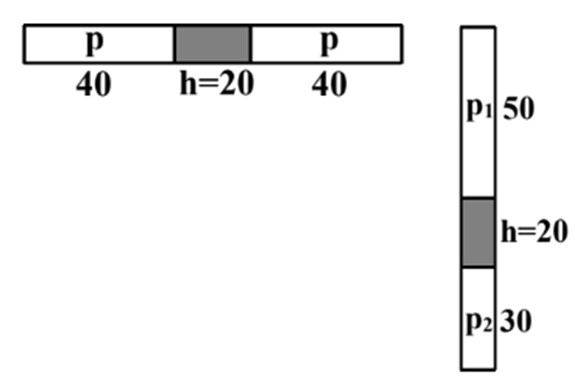
\includegraphics[width=0.35\linewidth]{../figs/VN12-Y24-PH-SYL-010P-5}
\end{center}
Theo định luật Boyle:
$$\begin{cases}
	p\cdot40 S=p_1\cdot50S\\
	p\cdot40S=p_2\cdot30S
\end{cases}\Rightarrow \begin{cases}
p_1=0,8p\\
p_2=\dfrac{4p}{3}
\end{cases}$$
Khi đặt ống thẳng đứng thì cột thuỷ ngân cân bằng khi:
$$p_2=p_1+h\Rightarrow p=\SI{37.5}{\centi\meter Hg}.$$
}

\item \mkstar{3}\\
Một ống hình trụ hẹp, kín hai đầu, dài $\ell=\SI{105}{\centi\meter}$, đặt nằm ngang. Chính giữa ống có một cột thuỷ ngân dài $h=\SI{21}{\centi\meter}$, phần còn lại của ống chứa không khí ở áp suất $p_0=\SI{72}{\centi\meter Hg}$. Coi nhiệt độ không khí trong ống không thay đổi. Khi ống đặt thẳng đứng thì độ di chuyển của cột thuỷ ngân là
\begin{mcq}(4)
	\item $\SI{3}{\centi\meter}$.
	\item $\SI{4}{\centi\meter}$.
	\item $\SI{6}{\centi\meter}$.
	\item $\SI{2}{\centi\meter}$.
\end{mcq}
\hideall{
\textbf{Đáp án C.}\\
$$pV=\text{const}\Rightarrow \begin{cases}
	72\cdot42=p_1\left(42+x\right)\\
	72\cdot42=p_2\left(42-x\right)
\end{cases}\Rightarrow \begin{cases}
p_1=\dfrac{3024}{42+x}\\
\ \\
p_2=\dfrac{3024}{42-x}
\end{cases}.$$
Mà
$$p_2=p_1+h\Rightarrow x=\SI{6}{\centi\meter}.$$
}

\item \mkstar{3}\\
Một lượng không khí có thể tích $\SI{240}{\centi\meter^3}$ chứa trong một cylanh có piston đóng kín, tiết diện của piston là $\SI{24}{\centi\meter^2}$. Áp suất của không khí trong cylanh bằng áp suất không khí bên ngoài và bằng $\SI{100}{\kilo\pascal}$. Cần một lực bằng bao nhiêu để dịch chuyển piston $\SI{2}{\centi\meter}$ theo chiều làm thể tích khí giảm? Bỏ qua ma sát giữa piston và thành cylanh. Coi trong quá trình chuyển động nhiệt độ khí không đổi.
\begin{center}
	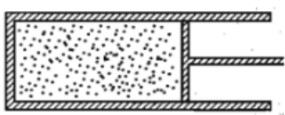
\includegraphics[width=0.25\linewidth]{../figs/VN12-Y24-PH-SYL-010P-3}
\end{center}
\begin{mcq}(4)
	\item $\SI{20}{\newton}$.
	\item $\SI{80}{\newton}$.
	\item $\SI{60}{\newton}$.
	\item $\SI{40}{\newton}$.
\end{mcq}
\hideall{
\textbf{Đáp án C.}\\
\begin{center}
	\begin{tabular}{C{4cm} C{3cm} C{4cm}}
		\colorbox{yellow}{\textcolor{red}{\textbf{Trạng thái 1}}} & $\xrightarrow[]{T_1=T_2}$ & \colorbox{yellow}{\textcolor{red}{\textbf{Trạng thái 2}}}\\
		$p_1=\SI{100}{\kilo\pascal}$ & &$p_2=?$\\
		$V_1=\SI{240}{\centi\meter^3}$ & & $V_2=\SI{192}{\centi\meter^3}$
	\end{tabular}
\end{center}
Theo định luật Boyle:
$$p_1V_1=p_2V_2\Rightarrow p_2=\SI{125}{\kilo\pascal}.$$
Piston cân bằng khi:
$$F+p_0S=p_2S\Rightarrow F=\left(p_2-p_0\right)S=\SI{60}{\newton}.$$
}

\item \mkstar{3}\\
Một bơm xe đạp hình trụ có đường kính trong là $\SI{3}{\centi\meter}$. Người ta dùng ngón tay bịt kín đầu vòi bơm và ấn piston từ từ để nén không khí trong bơm sao cho nhiệt độ không thay đổi. Lấy áp suất khí quyển là $p_0=\SI{E5}{\pascal}$. Để thể tích của không khí trong bơm giảm đi 4 lần thì lực tác dụng lên piston là
\begin{mcq}(4)
	\item $\SI{250}{\newton}$.
	\item $\SI{225}{\newton}$.
	\item $\SI{200}{\newton}$.
	\item $\SI{212}{\newton}$.
\end{mcq}
\hideall{
\textbf{Đáp án D.}\\
Theo định luật Boyle:
$$p_0V_0=p\dfrac{V_0}{4}\Rightarrow p=4p_0.$$
Để piston cân bằng:
$$F+p_0S=pS\Rightarrow F=\left(p-p_0\right)S=3p_0\cdot\pi\dfrac{d^2}{4}\approx\SI{212}{\newton}.$$
}

\item \mkstar{3}\\
Cylanh và piston nhẹ cách nhiệt chứa bên trong nó một lượng khí xác định. Ban đầu thể tích khí chứa trong cylanh là $\SI{1000}{\centi\meter^3}$. Tiến hành đặt lên piston một gia trọng có khối lượng $\SI{10}{\kilogram}$. Biết tiết diện của piston là $S=\SI{100}{\centi\meter^2}$, lấy $g=\SI{10}{\meter/\second^2}$, áp suất khí quyển $p_0=\SI{E5}{\pascal}$. Thể tích của khí trong cylanh khi piston cân bằng là
\begin{center}
	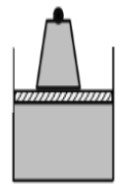
\includegraphics[width=0.1\linewidth]{../figs/VN12-Y24-PH-SYL-010P-4}
\end{center}
\begin{mcq}(4)
	\item $\SI{910}{\centi\meter^3}$.
	\item $\SI{1100}{\centi\meter^3}$.
	\item $\SI{800}{\centi\meter^3}$.
	\item $\SI{600}{\centi\meter^3}$.
\end{mcq}
\hideall{
\textbf{Đáp án A.}\\
\begin{center}
	\begin{tabular}{C{4cm} C{3cm} C{4cm}}
		\colorbox{yellow}{\textcolor{red}{\textbf{Trạng thái 1}}} & $\xrightarrow[]{T_1=T_2}$ & \colorbox{yellow}{\textcolor{red}{\textbf{Trạng thái 2}}}\\
		$p_1=\SI{E5}{\pascal}$ & &$p_2=p_0+\dfrac{mg}{S}=\SI{1.1E5}{\pascal}$\\
		$V_1=\SI{1000}{\centi\meter^3}$ & & $V_2=?$
	\end{tabular}
\end{center}
Theo định luật Boyle:
$$p_1V_1=p_2V_2\Rightarrow V_2\approx\SI{910}{\centi\meter^3}.$$
}

\item\mkstar{4}\\
Ở chính giữa một ống thuỷ tinh nằm ngang, kín cả hai đầu có một cột thuỷ ngân dài $h=\SI{19.6}{\centi\meter}$. Nếu đặt ống nghiêng một góc $\SI{30}{\degree}$ so với phương nằm ngang thì cột thuỷ ngân dịch chuyển một đoạn $\Delta \ell_1=\SI{20}{\milli\meter}$. Nếu đặt ống thẳng đứng thì cột thuỷ ngân dịch chuyển một đoạn $\Delta \ell_2=\SI{30}{\milli\meter}$. Coi nhiệt độ không khí không thay đổi. Áp suất của không khí trong ống khi ống nằm ngang gần bằng
\begin{mcq}(4)
	\item $\SI{19}{\milli\meter Hg}$.
	\item $\SI{6}{\milli\meter Hg}$.
	\item $\SI{10}{\milli\meter Hg}$.
	\item $\SI{30}{\milli\meter Hg}$.
\end{mcq}
\hideall{
\textbf{Đáp án C.}\\
\begin{center}
	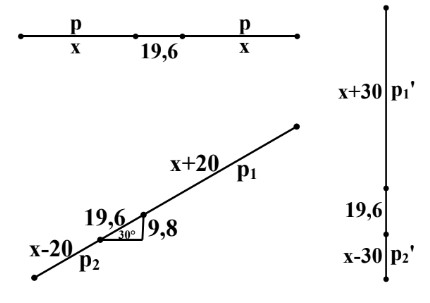
\includegraphics[width=0.35\linewidth]{../figs/VN12-Y24-PH-SYL-010P-6}
\end{center}
Theo định luật Boyle:
$$pV=\text{const}\Rightarrow \begin{cases}
	px=p_1\left(20+x\right)=p'_1\left(30+x\right)\\
	px=p_2\left(x-20\right)=p'_2\left(x-30\right)
\end{cases}$$
Lại có
$$\begin{cases}
	p_2=p_1+19,6\sin\SI{30}{\degree}\\
	p'_2=p'_1+19,6
\end{cases}\Rightarrow \begin{cases}
p_2-p_1=9,8\\
p'_2-p'_1=19,6
\end{cases}$$
$$\Rightarrow\begin{cases}
	\dfrac{px}{x-20}-\dfrac{px}{x+20}=9,8\\
	\ \\
	\dfrac{px}{x-30}-\dfrac{px}{x+30}=19,6
\end{cases}\Rightarrow \begin{cases}
p\approx\SI{10}{\milli\meter Hg}\\
x\approx\SI{48.99}{\milli\meter}
\end{cases}.$$
}

\item \mkstar{4}\\
Một ống thuỷ tinh được cắm lộn ngược vào một chậu thuỷ ngân, bên trong ống chứa $\SI{40}{\centi\meter^3}$ không khí và một cột thuỷ ngân cao $\SI{8}{\centi\meter}$ so với mực thuỷ ngân trong chậu (hình a). Người ta ấn sâu ống thuỷ tinh vào thuỷ ngân cho tới khi mực thuỷ ngân ở bên trong và bên ngoài ống bằng nhau (hình b). Biết áp suất khí quyển là $\SI{75}{\centi\meter Hg}$. Xem nhiệt độ không khí trong ống không thay đổi. Thể tích của không khí còn lại bên trong ống lúc sau là
\begin{center}
	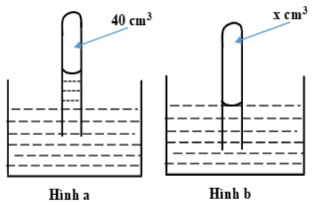
\includegraphics[width=0.35\linewidth]{../figs/VN12-Y24-PH-SYL-010P-7}
\end{center}
\begin{mcq}(4)
	\item $\SI{44.78}{\centi\meter^3}$.
	\item $\SI{35.7}{\centi\meter^3}$.
	\item $\SI{44.27}{\centi\meter^3}$.
	\item $\SI{36.14}{\centi\meter^3}$.
\end{mcq}
\hideall{
\textbf{Đáp án B.}\\
\begin{center}
	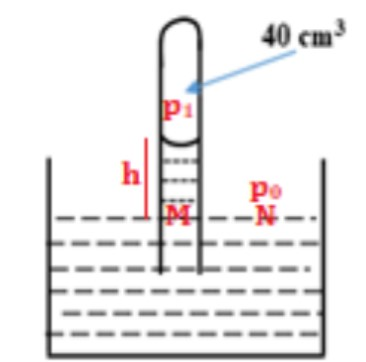
\includegraphics[width=0.2\linewidth]{../figs/VN12-Y24-PH-SYL-010P-8}
\end{center}
Hình a có áp suất tại hai điểm M và N trên mặt phẳng nằm ngang bằng nhau:
$$p_\text{M}=p_\text{N}\Rightarrow p_1+h=p_0\Rightarrow p_1=p_0-h=\SI{67}{\centi\meter Hg}.$$
Tương tự ở hình b có $p_2=p_0=\SI{75}{\centi\meter Hg}$.\\
Theo định luật Boyle:
$$p_1V_1=p_2V_2\Rightarrow V_2\approx\SI{35.7}{\centi\meter^3}.$$
}


\end{enumerate}

\section{Trắc nghiệm đúng/sai}
\begin{enumerate}[label=\bfseries Câu \arabic*:, leftmargin=1.7cm]
	\item \mkstar{1}\\
	Khi nén đẳng nhiệt một lượng khí lí tưởng xác định thì
	\begin{enumerate}[label=\alph*)]
		\item thể tích khí giảm.
		\item áp suất khí tăng.
		\item số phân tử khí giảm.
		\item mật độ phân tử khí tăng.
	\end{enumerate}
\hideall{
\begin{enumerate}[label=\alph*)]
	\item Đúng.
	\item Đúng.
	\item Sai. Số phân tử khí không đổi.
	\item Đúng.
\end{enumerate}
}

\item\mkstar{3}\\
Một khối khí lí tưởng ban đầu ở điều kiện tiêu chuẩn (trạng thái A). Nén khí và giữ nhiệt độ không đổi đến trạng thái B. Đồ thị áp suất theo thể tích được biểu diễn như hình vẽ bên
\begin{center}
	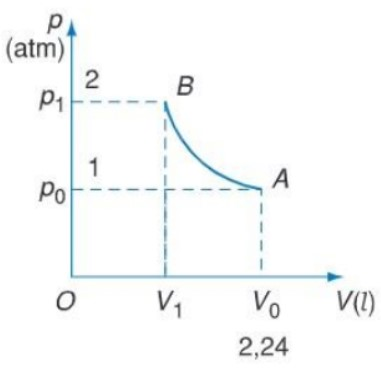
\includegraphics[width=0.35\linewidth]{../figs/VN12-Y24-PH-SYL-010P-11}
\end{center}
\begin{enumerate}[label=\alph*)]
	\item Số mol của khối khí trên là $\SI{0.1}{\mole}$.
	\item Đường biểu diễn quá trình nén đẳng nhiệt trong đồ thị trên là một cung hyperbol.
	\item Thể tích khí ở trạng thái B là $\SI{1.12}{\liter}$.
	\item Khi thể tích khối khí là $\SI{1.4}{\liter}$ thì áp suất khí là $\SI{3.136}{atm}$.
\end{enumerate}
\hideall{
\begin{enumerate}[label=\alph*)]
	\item Đúng.
	\item Đúng.
	\item Đúng.
	\item Sai. Áp suất khí khi thể tích khí $\SI{1.4}{\liter}$ là $\SI{1.6}{atm}$.
\end{enumerate}
}

\item \mkstar{3}\\
Một quả bóng thể tích $\SI{0.5}{\meter^3}$ được nối với một quả cầu sắt khối lượng $\SI{2.5E2}{\kilogram}$ và được ném xuống hồ nước. Quả bóng được làm từ vật liệu nhẹ và độ đàn hồi không đáng kể (mặc dù nó có thể bị nén). Ban đầu không khí trong bóng có áp suất bằng áp suất khí quyển bằng $\SI{1.01E5}{\pascal}$. Biết rằng khối lượng riêng của sắt, không khí và nước lần lượt  là $\SI{7.86E3}{\kilogram/\meter^3}$, $\SI{1.29}{\kilogram/\meter^3}$, $\SI{1000}{\kilogram/\meter^3}$. Xem rằng nhiệt độ quả bóng trong quá trình chìm vẫn không đổi.
\begin{enumerate}[label=\alph*)]
	\item Áp suất và thể tích của khí trong quả bóng tuân theo định luật Boyle.
	\item Thể tích quả bóng ở vị trí cân bằng là $\SI{0.218}{\meter^3}$.
	\item Áp suất không khí trong quả bóng tại vị trí cân bằng là $\SI{2.31E5}{\pascal}.$
	\item Độ sâu quả bóng đạt được tại vị trí cân bằng là $\SI{13.3}{\meter}$.
\end{enumerate}
\hideall{
\begin{enumerate}[label=\alph*)]
	\item Đúng.
	\item Sai.
	\begin{eqnarray}
		V_{\ce{Fe}}&=&\dfrac{m_{\ce{Fe}}}{\rho_{\ce{Fe}}}=\SI{0.0318}{\meter^3}\\
		m_\text{b}&=&\rho_\text{kk}V_\text{b}=\SI{0.645}{\kilogram}
	\end{eqnarray}
Quả bóng cân bằng khi:
$$m_\text{b}g+m_{\ce{Fe}}g=\rho_\text{n}g\left(V_\text{b}+V_{\ce{Fe}}\right)\Rightarrow V_\text{b}=\dfrac{m_\text{b}+m_{\ce{Fe}-\rho_\text{n}V_{\ce{Fe}}}}{\rho_\text{n}}=\SI{0.219}{\meter^3} .$$
\item Đúng.
$$p_0V_0=p_\text{b}V_\text{b}\Rightarrow p_\text{b}=\SI{2.31E5}{\pascal}.$$
\item Đúng.
$$p_\text{b}=p_0+\rho_\text{n}gh\Rightarrow h=\SI{13.3}{\meter}.$$
\end{enumerate}
}
\end{enumerate}
\section{Bài tập tự luận}
\begin{enumerate}[label=\bfseries Câu \arabic*:, leftmargin=1.7cm]
	
	\item\mkstar{2}\\
	Để tăng thể tích của một khối lượng khí nhất định lên $\SI{10}{\percent}$ ở nhiệt độ không đổi thì cần giảm áp suất khí bao nhiêu $\si{\percent}$?
	\hideall{
$$\dfrac{p_2}{p_1}=\dfrac{V_1}{V_2}=\dfrac{1}{1,1}\approx\SI{90.9}{\percent}\Rightarrow\Delta p\approx\SI{9.1}{\percent}p_1.$$	
}

\item \mkstar{2}\\
Quá trình biến đổi trạng thái của một lượng khí lí tưởng xác định được biểu diễn bằng đồ thị hình vẽ. Biết ở trạng thái (1) khí có thể tích $\SI{100}{\centi\meter^3}$. Thể tích khí tại trạng thái (2) là bao nhiêu?
\begin{center}
	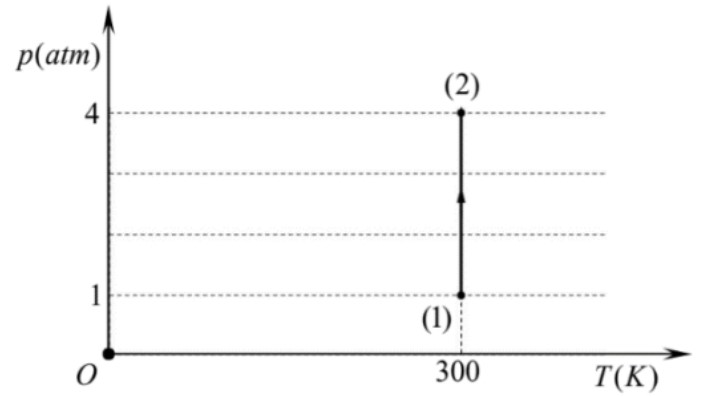
\includegraphics[width=0.45\linewidth]{../figs/VN12-Y24-PH-SYL-010P-1}
\end{center}
\hideall{
$$p_1V_1=p_2V_2\Rightarrow V_2=\SI{25}{\centi\meter^3}.$$
}

\item\mkstar{2}\\
Quá trình biến đổi trạng thái của một lượng khí xác định được biểu diễn bằng đồ thị hình vẽ. Áp suất của chất khí tại trạng thái (2) bằng bao nhiêu?
\begin{center}
	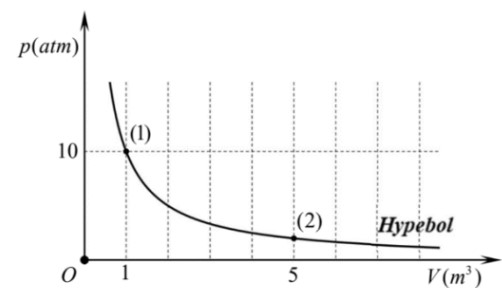
\includegraphics[width=0.45\linewidth]{../figs/VN12-Y24-PH-SYL-010P-2}
\end{center}
\hideall{
$$p_1V_1=p_2V_2\Rightarrow p_2=\SI{2}{atm}.$$
}

\item \mkstar{2}\\
Người ta điều chế khí hydrogen và chứa vào một bình lớn dưới áp suất $\SI{1}{atm}$. Tính thể tích khí phải lấy ra từ bình lớn để nạp vào bình nhỏ có thể tích $\SI{20}{\liter}$ ở áp suất $\SI{25}{atm}$. Coi quá trình nạp khí là đẳng nhiệt.
\hideall{
\begin{center}
	\begin{tabular}{C{4cm} C{3cm} C{4cm}}
		\colorbox{yellow}{\textcolor{red}{\textbf{Trạng thái 1}}} & $\xrightarrow[]{T_1=T_2}$ & \colorbox{yellow}{\textcolor{red}{\textbf{Trạng thái 2}}}\\
		$p_1=\SI{1}{atm}$ & &$p_2=\SI{25}{atm}$\\
		$V_1=?$ & & $V_2=\SI{20}{\liter}$
	\end{tabular}
\end{center}
Theo định luật Boyle:
$$p_1V_1=p_2V_2\Rightarrow V_1=\SI{500}{\liter}.$$

}

\item \mkstar{2}\\
Người ta nén đẳng nhiệt $\SI{3}{\gram}$ khí hydrogen ở điều kiện tiêu chuẩn $\left(p_0=\SI{1}{atm},\ T_0=\SI{273}{\kelvin}\right)$ đến áp suất $\SI{2}{atm}$. Thể tích của lượng khí đó sau khi biến đổi là bao nhiêu?
\hideall{
\begin{center}
	\begin{tabular}{C{4cm} C{3cm} C{4cm}}
		\colorbox{yellow}{\textcolor{red}{\textbf{Trạng thái 1}}} & $\xrightarrow[]{T_1=T_2}$ & \colorbox{yellow}{\textcolor{red}{\textbf{Trạng thái 2}}}\\
		$p_1=\SI{1}{atm}$ & &$p_2=\SI{2}{atm}$\\
		$V_1=\dfrac{m}{M}\cdot\left(\SI{22.4}{\liter}\right)=\SI{33.6}{\liter}$ & & $V_2=?$
	\end{tabular}
\end{center}
Theo định luật Boyle:
$$p_1V_1=p_2V_2\Rightarrow V_2=\SI{16.8}{\liter}.$$
}

\item \mkstar{2}\\
Một khối khí ở $\SI{0}{\celsius}$ và áp suất $\SI{10}{atm}$ có thể tích $\SI{10}{\liter}$. Hỏi thể tích của khối khí ở điều kiện tiêu chuẩn là bao nhiêu?
\hideall{
$\SI{100}{\liter}.$
}

\item\mkstar{2}\\
Một khối khí xác định dãn nở đẳng nhiệt từ thể tích ban đầu $\SI{5}{\liter}$ đến $\SI{12}{\liter}$ thì áp suất khối khí đã giảm một lượng $\SI{80}{\kilo\pascal}$. Áp suất ban đầu của khối khí bằng bao nhiêu?
\hideall{
\begin{center}
	\begin{tabular}{C{4cm} C{3cm} C{4cm}}
		\colorbox{yellow}{\textcolor{red}{\textbf{Trạng thái 1}}} & $\xrightarrow[]{T_1=T_2}$ & \colorbox{yellow}{\textcolor{red}{\textbf{Trạng thái 2}}}\\
		$p_1=?$ & &$p_2=p_1-\SI{80}{\kilo\pascal}$\\
		$V_1=\SI{5}{\liter}$ & & $V_2=\SI{12}{\liter}$
	\end{tabular}
\end{center}
Theo định luật Boyle:
$$p_1V_1=p_2V_2\Leftrightarrow p_1\cdot5=\left(p_1-80\right)\cdot12\Rightarrow p_1=\SI{137.14}{\kilo\pascal}.$$
}

\item \mkstar{2}\\
Khối lượng riêng của không khí ở điều kiện chuẩn $\left(p=\SI{1}{atm},\ t=\SI{0}{\celsius}\right)$ là $\SI{1.28}{\kilogram/\meter^3}$. Hỏi ở áp suất bao nhiêu thì khối lượng riêng của không khí là $\SI{0.64}{\kilogram/\meter^3}$. Biết rằng nhiệt độ không khí không đổi.
\hideall{
$$\dfrac{p_2}{p_1}=\dfrac{V_1}{V_2}=\dfrac{\rho_2}{\rho_1}\Rightarrow p_2=\SI{0.5}{atm}.$$
}

\item Dùng một bơm hơi dung tích $\SI{1.5}{\liter}$ để bơm cho một chiếc săm dung tích $\SI{5}{\liter}$. Hỏi cần phải bơm bao nhiêu lần để áp suất trong săm đạt $\SI{4}{atm}$. Biết rằng ban đầu không khí trong săm cũng có áp suất bằng áp suất khí quyển và bằng $\SI{1}{atm}$. Coi nhiệt độ không khí không đổi trong quá trình bơm.
\hideall{
10 lần.
}

\item \mkstar{3}\\
Ống thuỷ tinh một đầu kín dài $\SI{112.2}{\centi\meter}$, chứa không khí ở áp suất khí quyển $p_0=\SI{75}{\milli\meter Hg}$. Ấn ống xuống một chậu nước theo phương thẳng đứng, miệng ống ở dưới. Khi đáy ống ngang với mặt nước thì độ cao cột nước đi vào ống bằng bao nhiêu? Biết rằng khối lượng riêng của nước  và thuỷ ngân lần lượt là $\SI{1000}{\kilogram/\meter^3}$ và $\SI{13600}{\kilogram/\meter^3}$. Biết rằng nhiệt độ không khí không đổi.
\hideall{
	Gọi $x$ là chiều cao cột nước đi vào trong ống.\\
	Áp suất không khí bên trong ống khi nhúng vào trong chậu nước:
	$$p+\dfrac{x\cdot\rho_{\ce{H_2O}}}{\rho_{\ce{Hg}}}=p_0+\dfrac{\ell\cdot\rho_{\ce{H_2O}}}{\rho_{\ce{Hg}}}\Rightarrow p=p_0+\dfrac{\left(\ell-x\right)\rho_{\ce{H_2O}}}{\rho_{\ce{Hg}}}=p_0+\dfrac{\ell-x}{13,6}.$$
	Theo định luật Boyle:
	$$p_0S\ell=\left(p_0+\dfrac{\ell-x}{13,6}\right)S\cdot\left(\ell-x\right)\Rightarrow x\approx\SI{10.2}{\centi\meter}.$$
}

\item \mkstar{3}\\
Ống thuỷ tinh một đầu kín dài $\SI{80}{\centi\meter}$, chứa không khí ở áp suất khí quyển $p_0=\SI{75}{\centi\meter Hg}$. Ấn ống xuống một chậu thuỷ ngân theo phương thẳng đứng, miệng ống ở dưới (thấp hơn) mặt thuỷ ngân $\SI{45}{\centi\meter}$. Độ cao cột thuỷ ngân đi vào ống bằng bao nhiêu? Biết rằng nhiệt độ không khí không đổi.
\hideall{Gọi $x$ là chiều cao cột thuỷ ngân đi vào trong ống.\\
Áp suất không khí trong ống sau khi nhúng ngập trong thuỷ ngân:
$$p+x=45+p_0\Rightarrow p=p_0+45-x.$$
Theo định luật Boyle:
$$p_0S\ell=\left(p_0+45-x\right)S\left(80-x\right)\Rightarrow x=\SI{20}{\centi\meter}.$$

}

\item \mkstar{3}\\
Một cylanh nằm ngang kín hai đầu, có thể tích $V=\SI{1.2}{\liter}$ và chứa không khí ở áp suất $p_0=\SI{E5}{\newton/\meter^2}$. Cylanh được chia thành 2 phần bằng nhau bởi piston mỏng khối lượng $m=\SI{100}{\gram}$ đặt thẳng đứng. Chiều dài cylanh $\SI{0.4}{\meter}$. Cylanh được quay với tốc độ góc $\omega$ quanh trục thẳng đứng ở giữa cylanh. Giá trị của $\omega$ bằng bao nhiêu nếu piston nằm cách trục quay đoạn $r=\SI{0.1}{\meter}$ khi có cân bằng tương đối? Biết rằng nhiệt độ khí trong cylanh là không đổi.
\hideall{
Áp dụng định luật Boyle cho mỗi ngăn khí:
$$\begin{cases}
	p_0V_0=p_1V_1\\
	p_0V_0=p_2V_2
\end{cases}\Rightarrow \begin{cases}
\left(\SI{E5}{\pascal}\right)\cdot\left(\SI{0.2}{\meter}\right)S=p_1\cdot\left(\SI{0.3}{\meter}\right)S\Rightarrow p_1=\xsi{\dfrac{2}{3}\cdot10^5}{\pascal}\\
\left(\SI{E5}{\pascal}\right)\cdot\left(\SI{0.2}{\meter}\right)S=p_2\cdot\left(\SI{0.1}{\meter}\right)S\Rightarrow p_2=\SI{2E5}{\pascal}
\end{cases}.$$
Tiết diện cylanh:
$$S=\dfrac{V}{\ell}=\SI{3E-3}{\meter^2}.$$
Khi piston đạt trạng thái cân bằng tương đối:
$$F_2-F_1=m\omega^2 r\Leftrightarrow \left(p_2-p_1\right)S=m\omega^2r\Rightarrow \omega =\SI{200}{\radian/\second}.$$
}

\item \mkstar{4}\\
Một phong vũ biểu chỉ sai vì có một ít không khí lọt vào ống. Ở áp suất khí quyển $p_0=\SI{755}{\milli\meter Hg}$ phong vũ biểu này chỉ $p_1=\SI{748}{\milli\meter Hg}$. Khi áp suất khí quyển là $p'_0=\SI{740}{\milli\meter Hg}$, phong vẽ biểu chỉ $p_2=\SI{736}{\milli\meter Hg}$. Coi diện tích mặt thuỷ ngân trong chậu lớn hơn nhiều so với tiết diện của ống, nhiệt độ không đổi. Chiều dài $\ell$ của ống phong vũ biểu bằng bao nhiêu?
\begin{center}
	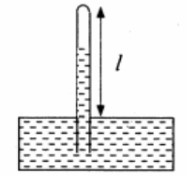
\includegraphics[width=0.2\linewidth]{../figs/VN12-Y24-PH-SYL-010P-9}
\end{center}
\hideall{
\begin{center}
	\begin{tabular}{C{6cm} C{2.5cm} C{6cm}}
		\colorbox{yellow}{\textcolor{red}{\textbf{Trạng thái 1}}} & $\xrightarrow[]{T_1=T_2}$ & \colorbox{yellow}{\textcolor{red}{\textbf{Trạng thái 2}}}\\
		$p_1=\SI{755}{\milli\meter Hg}-\SI{748}{\milli\meter Hg}=\SI{7}{\milli\meter Hg}$ & &$p_2=\SI{740}{\milli\meter Hg}-\SI{736}{\milli\meter Hg}=\SI{4}{\milli\meter Hg}$\\
		$V_1=S\left(\ell-748\right)$ & & $V_2=S\left(\ell-736\right)$
	\end{tabular}
\end{center}
Theo định luật Boyle:
$$p_1V_1=p_2V_2\Rightarrow \ell=\SI{764}{\milli\meter Hg}.$$
}


\item \mkstar{4}\\
Một ống thuỷ tinh có chiều dài $\ell=\SI{50}{\centi\meter}$, tiết diện $S=\SI{0.5}{\centi\meter^2}$, được hàn kín một đầu và chứa đầy không khí. Biết khối lượng ống $m=\SI{15}{\gram}$, áp suất khí quyển $p_0=\SI{760}{\milli\meter Hg}$ và nhiệt độ không khí trong ống là không đổi. Ấn ống chìm vào trong nước theo phương thẳng đứng, đầu kín ở trên. Để giữ ống trong nước sao cho đầu trên của ống thấp hơn mặt nước một đoạn $h=\SI{10}{\centi\meter}$ thì lực ấn cần đặt lên ống bằng bao nhiêu?
\hideall{
	Gọi $x$ là chiều cao cột không khí trong ống khi nhúng ống thuỷ tinh vào trong nước.
	\begin{center}
		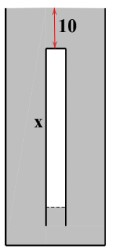
\includegraphics[width=0.1\linewidth]{../figs/VN12-Y24-PH-SYL-010P-10}
	\end{center}
\begin{center}
	\begin{tabular}{C{4cm} C{3cm} C{4cm}}
		\colorbox{yellow}{\textcolor{red}{\textbf{Trạng thái 1}}} & $\xrightarrow[]{T_1=T_2}$ & \colorbox{yellow}{\textcolor{red}{\textbf{Trạng thái 2}}}\\
		$p_1=\SI{76}{\centi\meter Hg}$ & &$p_2=76+\xsi{\dfrac{10+x}{13,6}}{\centi\meter Hg}$\\
		$V_1=S\ell=\SI{25}{\centi\meter^3}$ & & $V_2=Sx=\xsi{0,5x}{\centi\meter^3}$
	\end{tabular}
\end{center}
Theo định luật Boyle:
$$p_1V_1=p_2V_2\Rightarrow x\approx\SI{47.37}{\centi\meter}.$$
Độ lớn lực ấn lên ống:
$$F=\rho_{\ce{H_2O}}V-mg=\rho_{\ce{H_2O}}Sx-mg\approx\SI{0.09}{\newton}.$$

}

\item \mkstar{4}\\
Một bơm hút khí dung tích $\Delta V$. Phải bơm bao nhiêu lần để hút khí trong bình có thể tích $V$ từ áp suất $p_0$ đến áp suất $p$? Coi nhiệt độ không khí là không đổi.
\hideall{
\begin{itemize}
	\item Sau khi hút lần 1: $p_0V=p_1\left(V+\Delta V\right)\Rightarrow p_1=\dfrac{p_0V}{V+\Delta V}.$
	\item Sau khi hút lần 2: $p_1V=p_2\left(V+\Delta V\right)\Rightarrow p_2=\dfrac{p_1V}{V+\Delta V}=p_0\left(\dfrac{V}{V+\Delta V}\right)^2.$
	\item \dots
	\item Sau khi hút lần thứ $n$: $p_n=p_0\left(\dfrac{V}{V+\Delta V}\right)^n.$
\end{itemize}
Như vậy, khi đạt áp suất $p$ thì số lần đã bơm:
$$n=\ln\left(\dfrac{p}{p_0}\right)/\ln\left(\dfrac{V}{V+\Delta V}\right).$$
}
\end{enumerate}
